\Exhibit{Cds}{%
    Торренты сборников игр на компакт-дисках с играми Алексея Инкина\WithTr%
}

Эти скриншоты показывают торренты сборников игр на компакт-дисках,
на них есть игры Алексея Инкина: `Lehasoft Dyna' и `Lehasoft TankBattle'.
В списке игр они ближе к концу скриншотов
обоих дисков.

На одном из дисков написан год -- 2003.
На другом диске нет даты, но есть системные требования для игр,
характерные для 2003 года:

\ParagraphQuote{%
    Windows 95/98/xp , Pentium 166 MMX, 32 Mb RAM, Sound Blaster 16 compatible sound Card, mouse%
}

Сам торрент опубликован в январе 2010, когда Алексею Инкину было 24 года.
Для доказательства, что Алексей Инкин публиковал игры под названием `Lehasoft', см. \ExhibitRef{Lehasoft}.

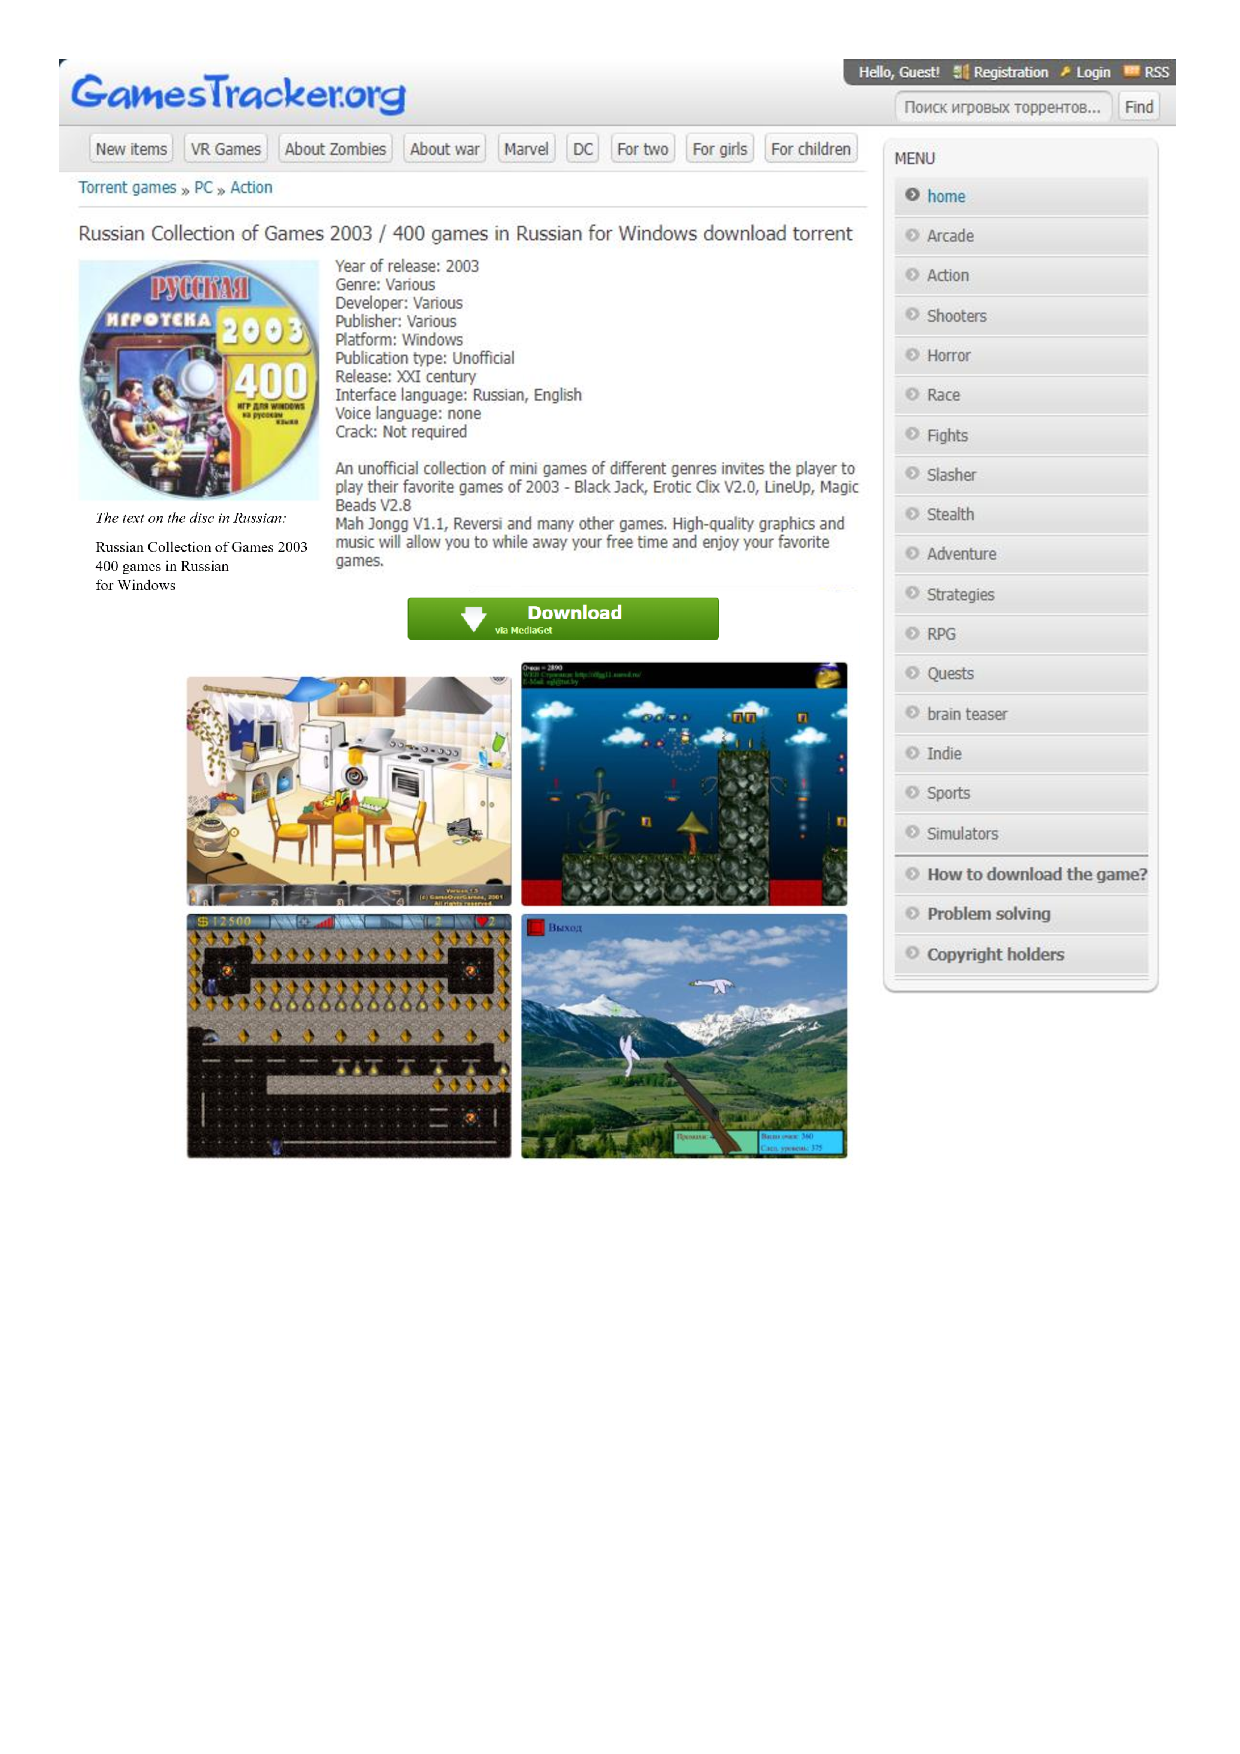
\includepdf[pages=-]{igroteka_eng_public}

\begin{center}
    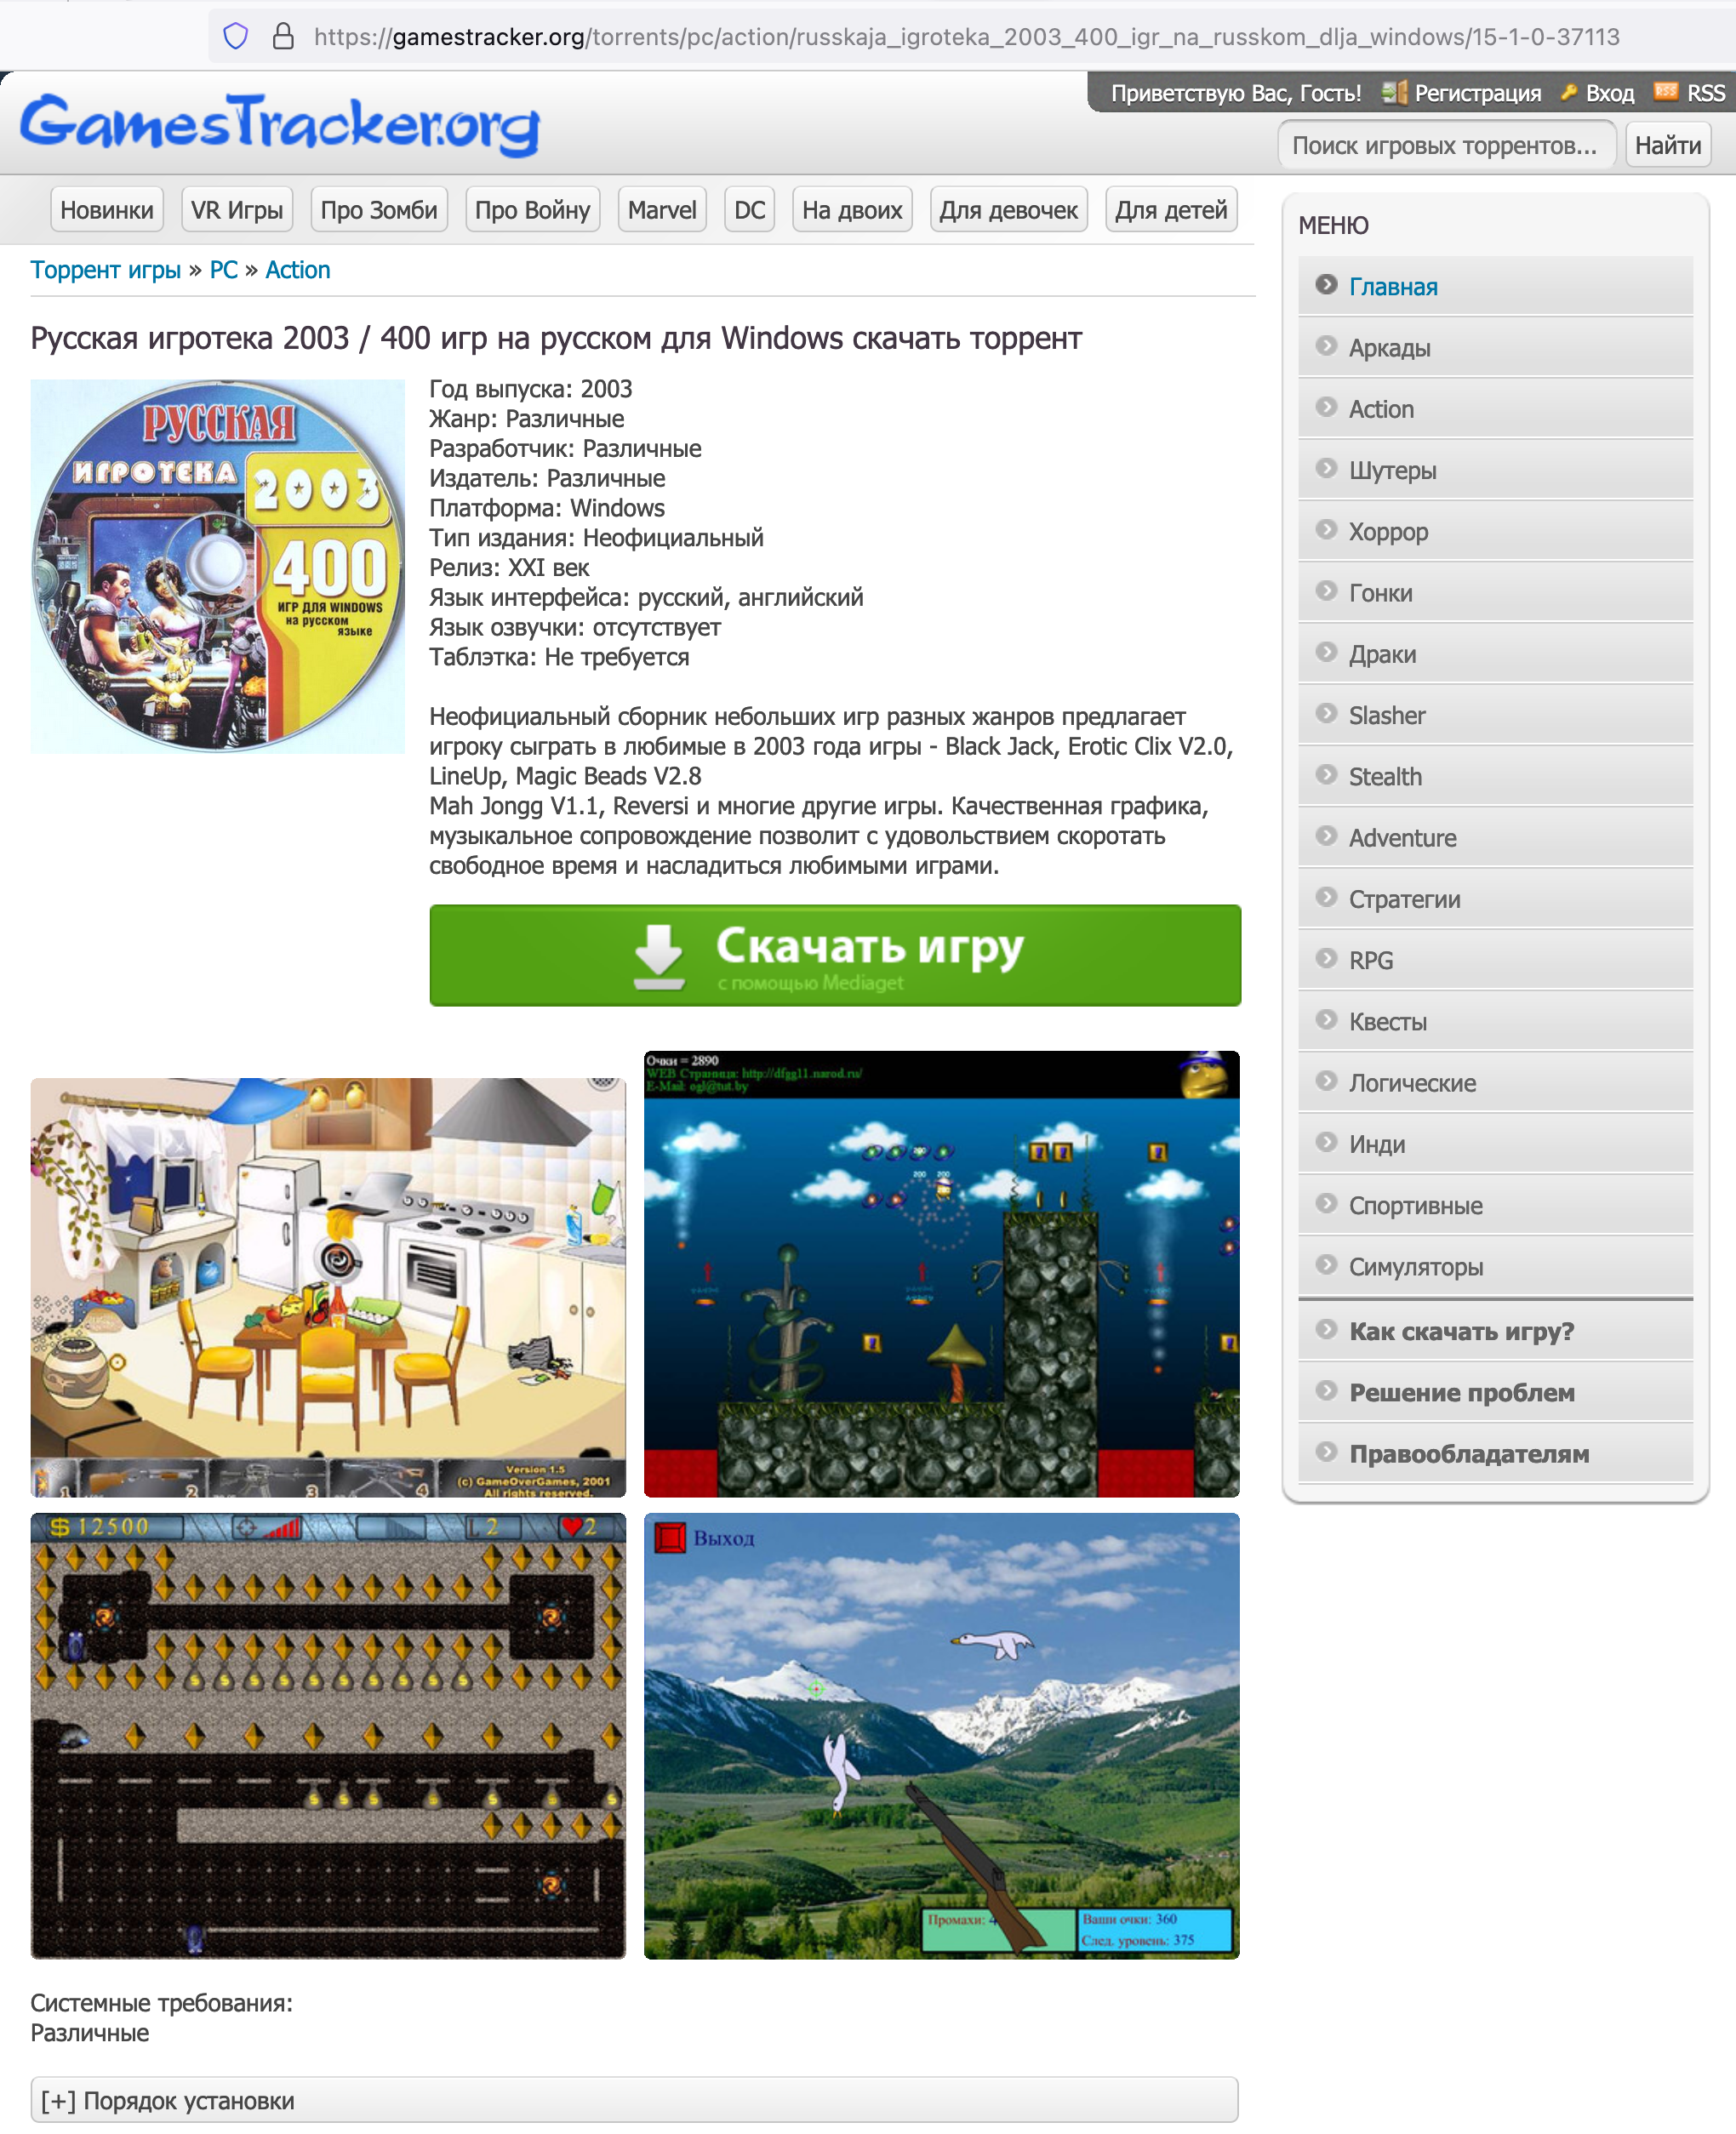
\includegraphics[width=\textwidth]{igroteka-p1}
\end{center}
\WillContinue
\pagebreak

\Continuing
\begin{center}
    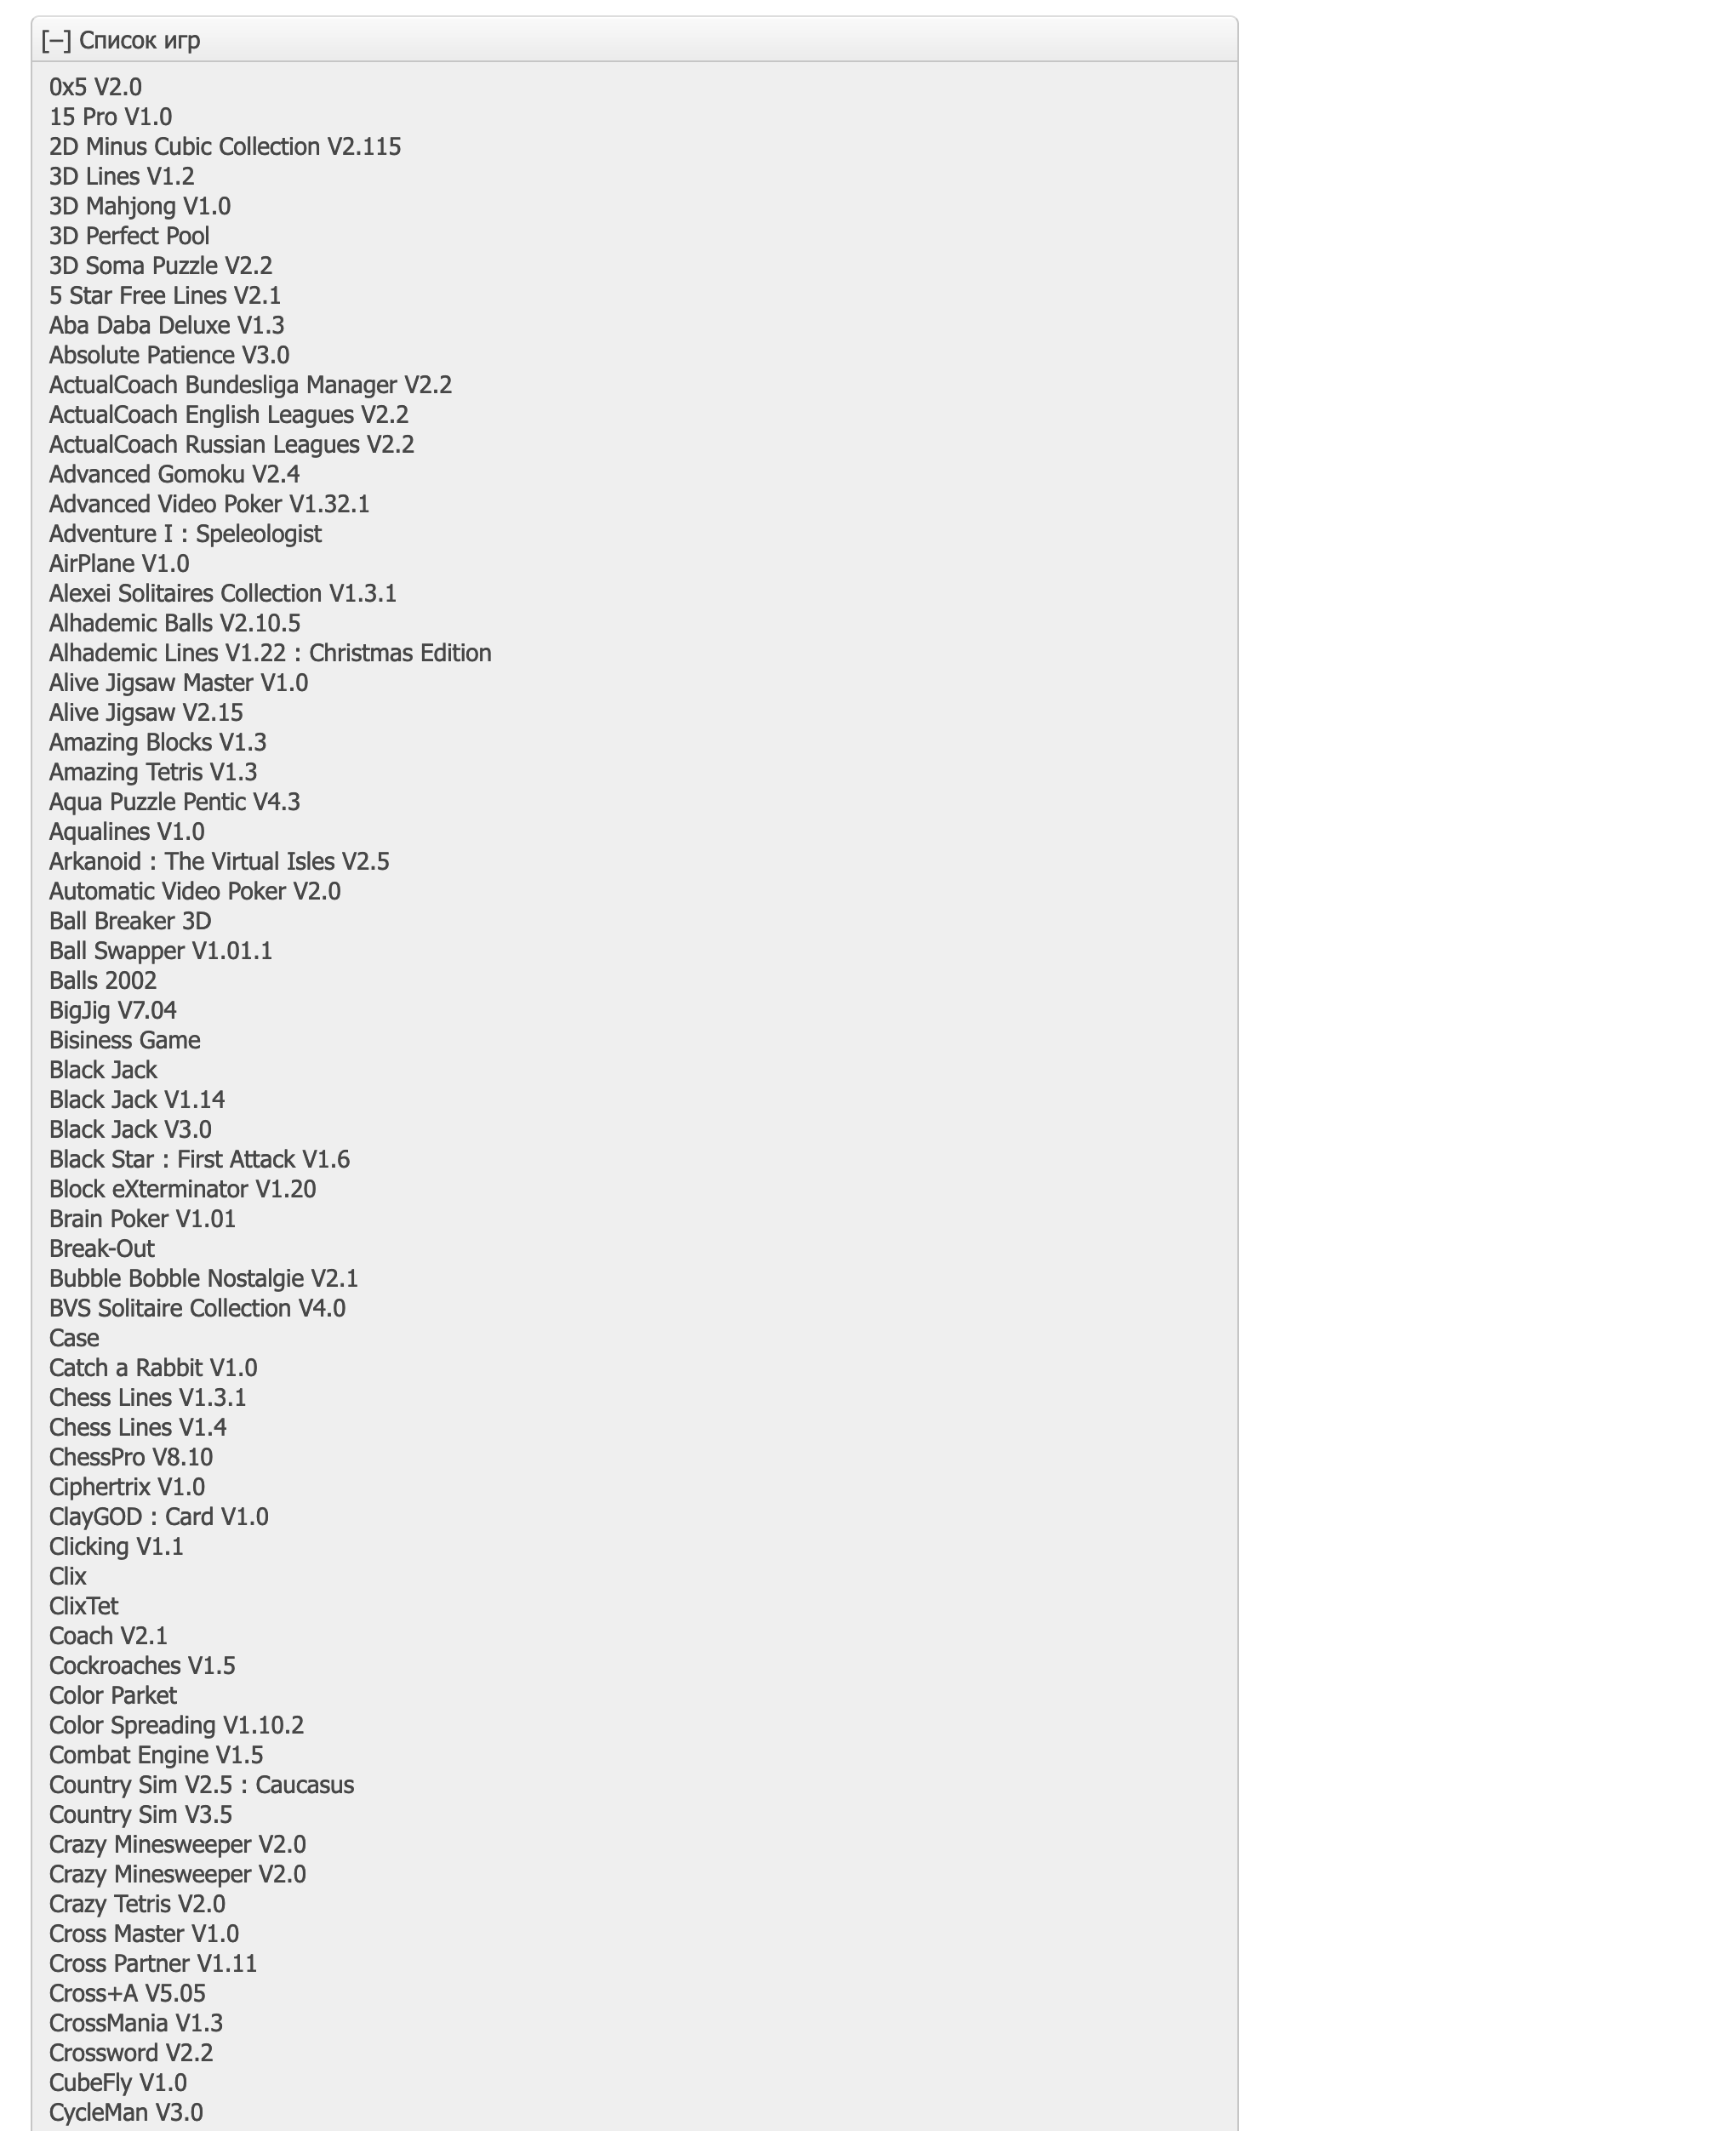
\includegraphics[width=\textwidth]{igroteka-p2}
\end{center}
\WillContinue
\pagebreak

\Continuing
\begin{center}
    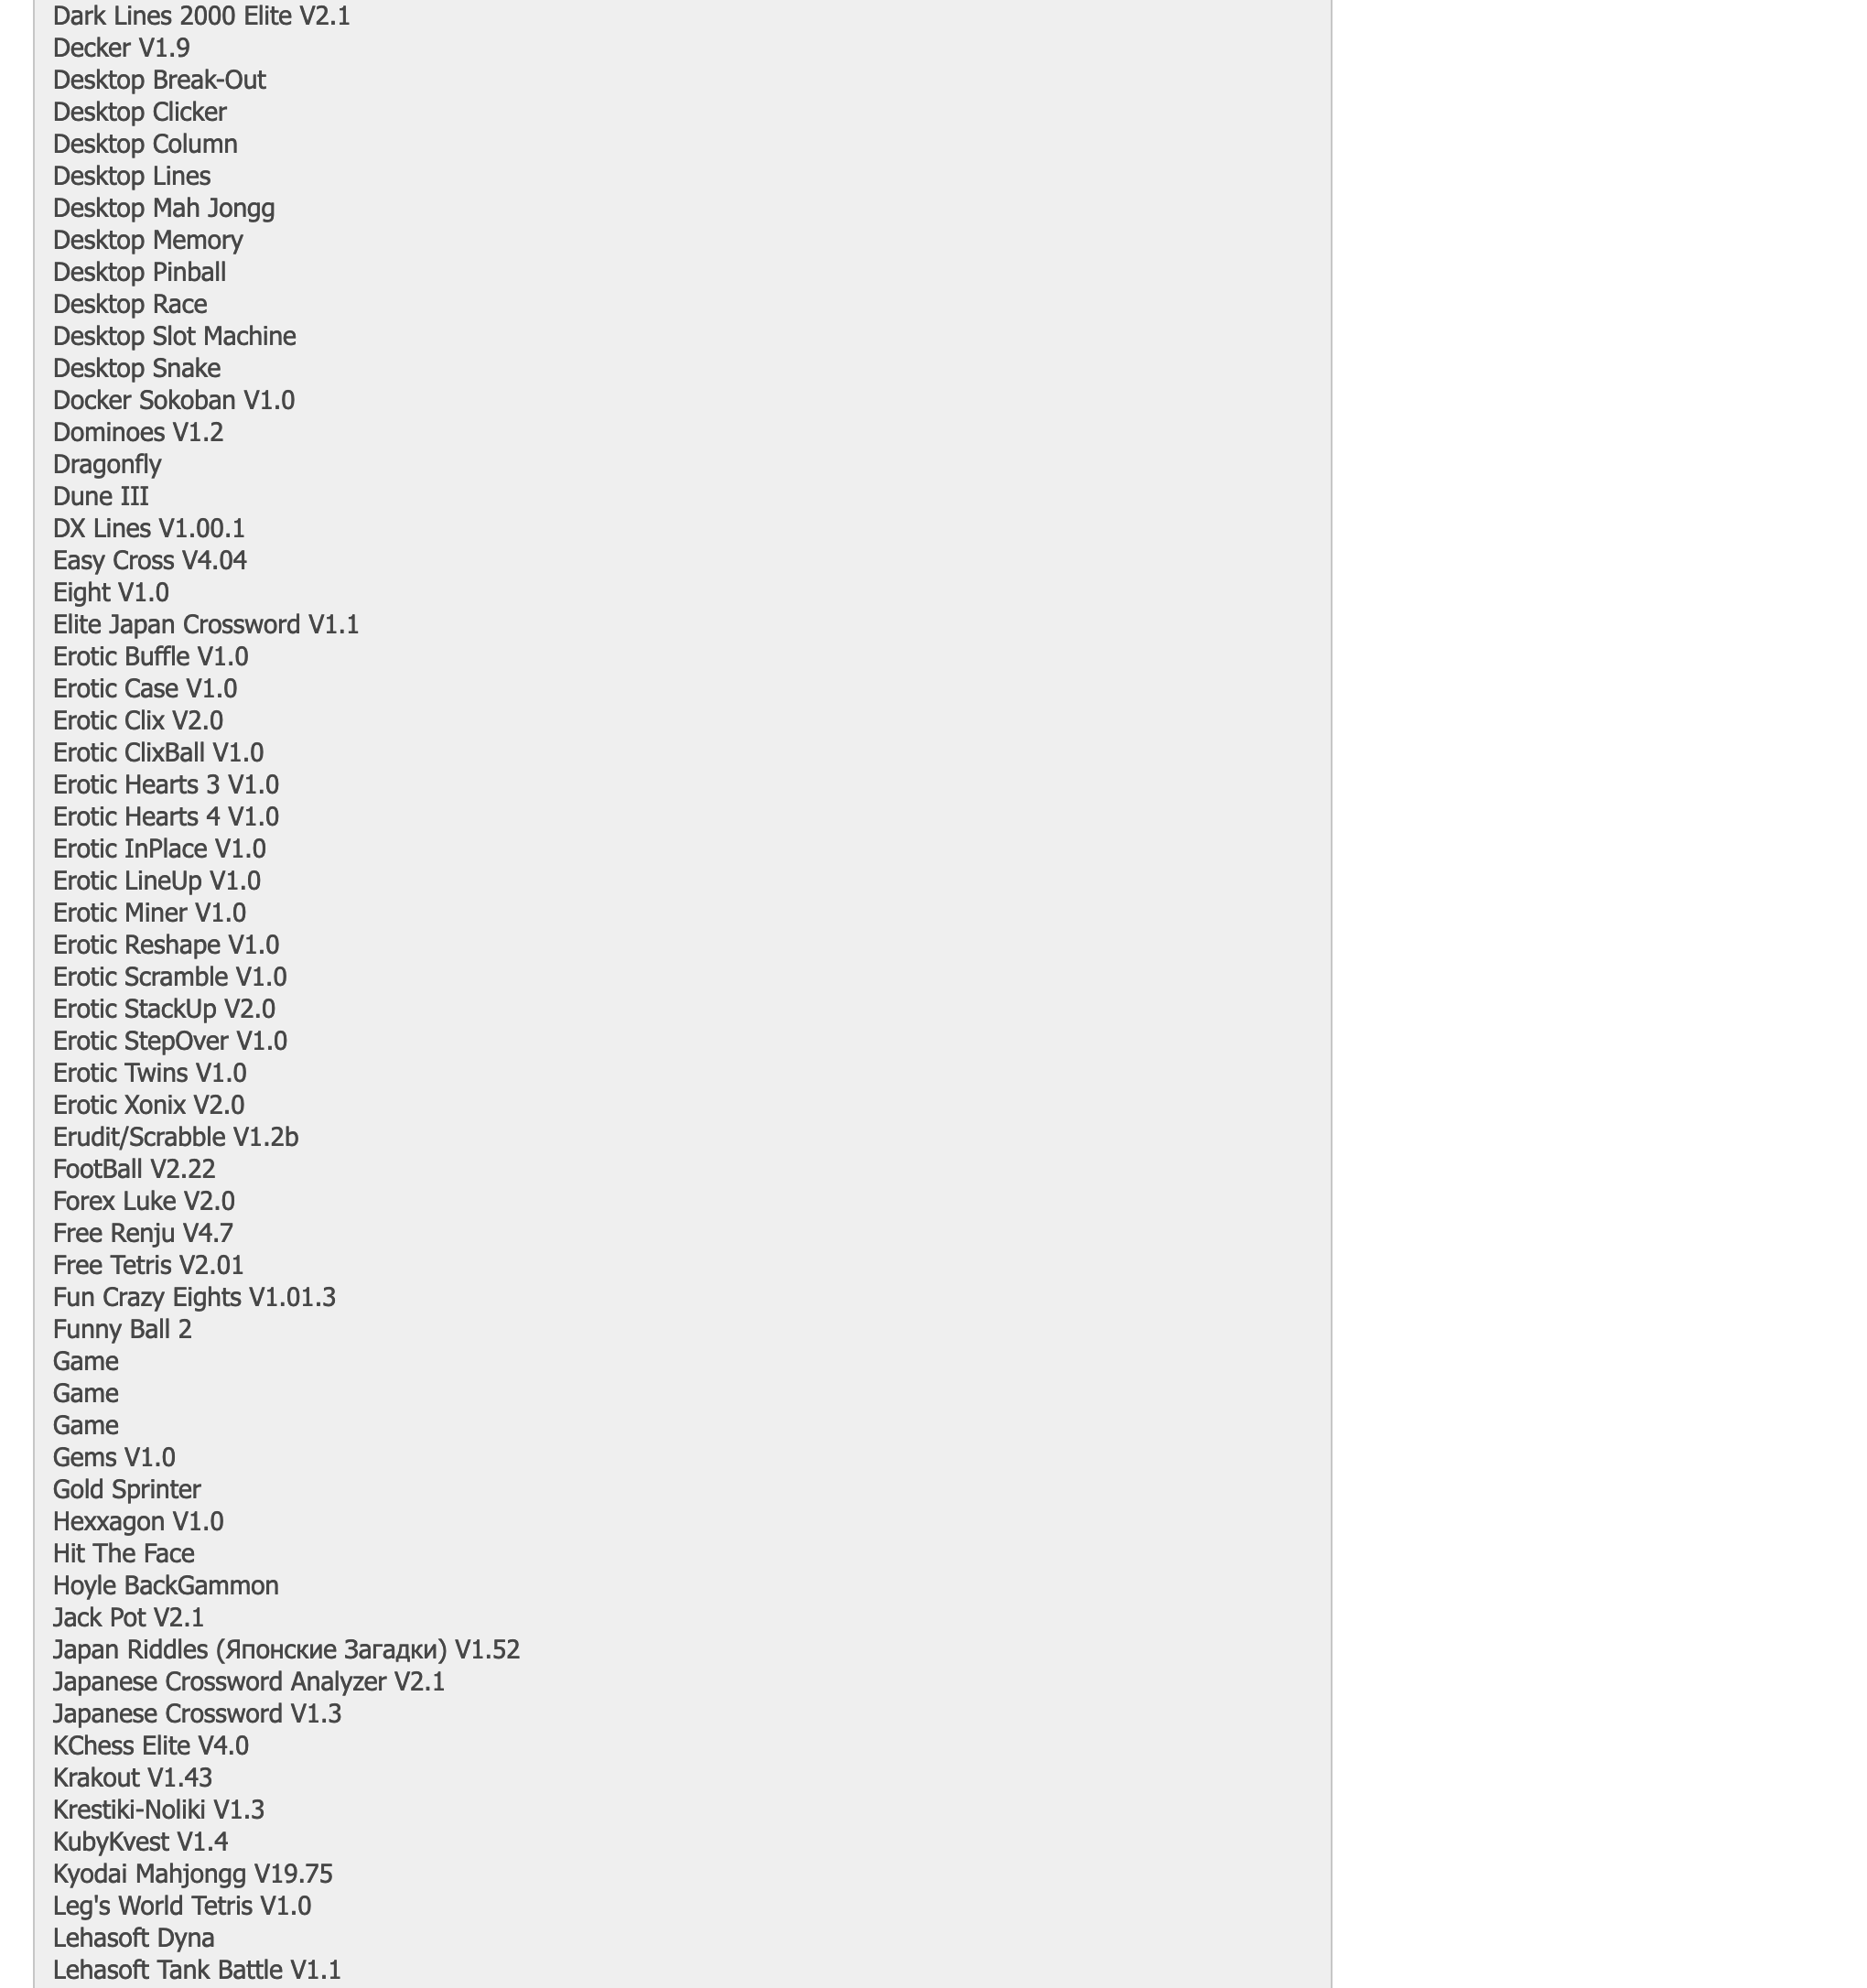
\includegraphics[width=\textwidth]{igroteka-p3}
\end{center}
\pagebreak

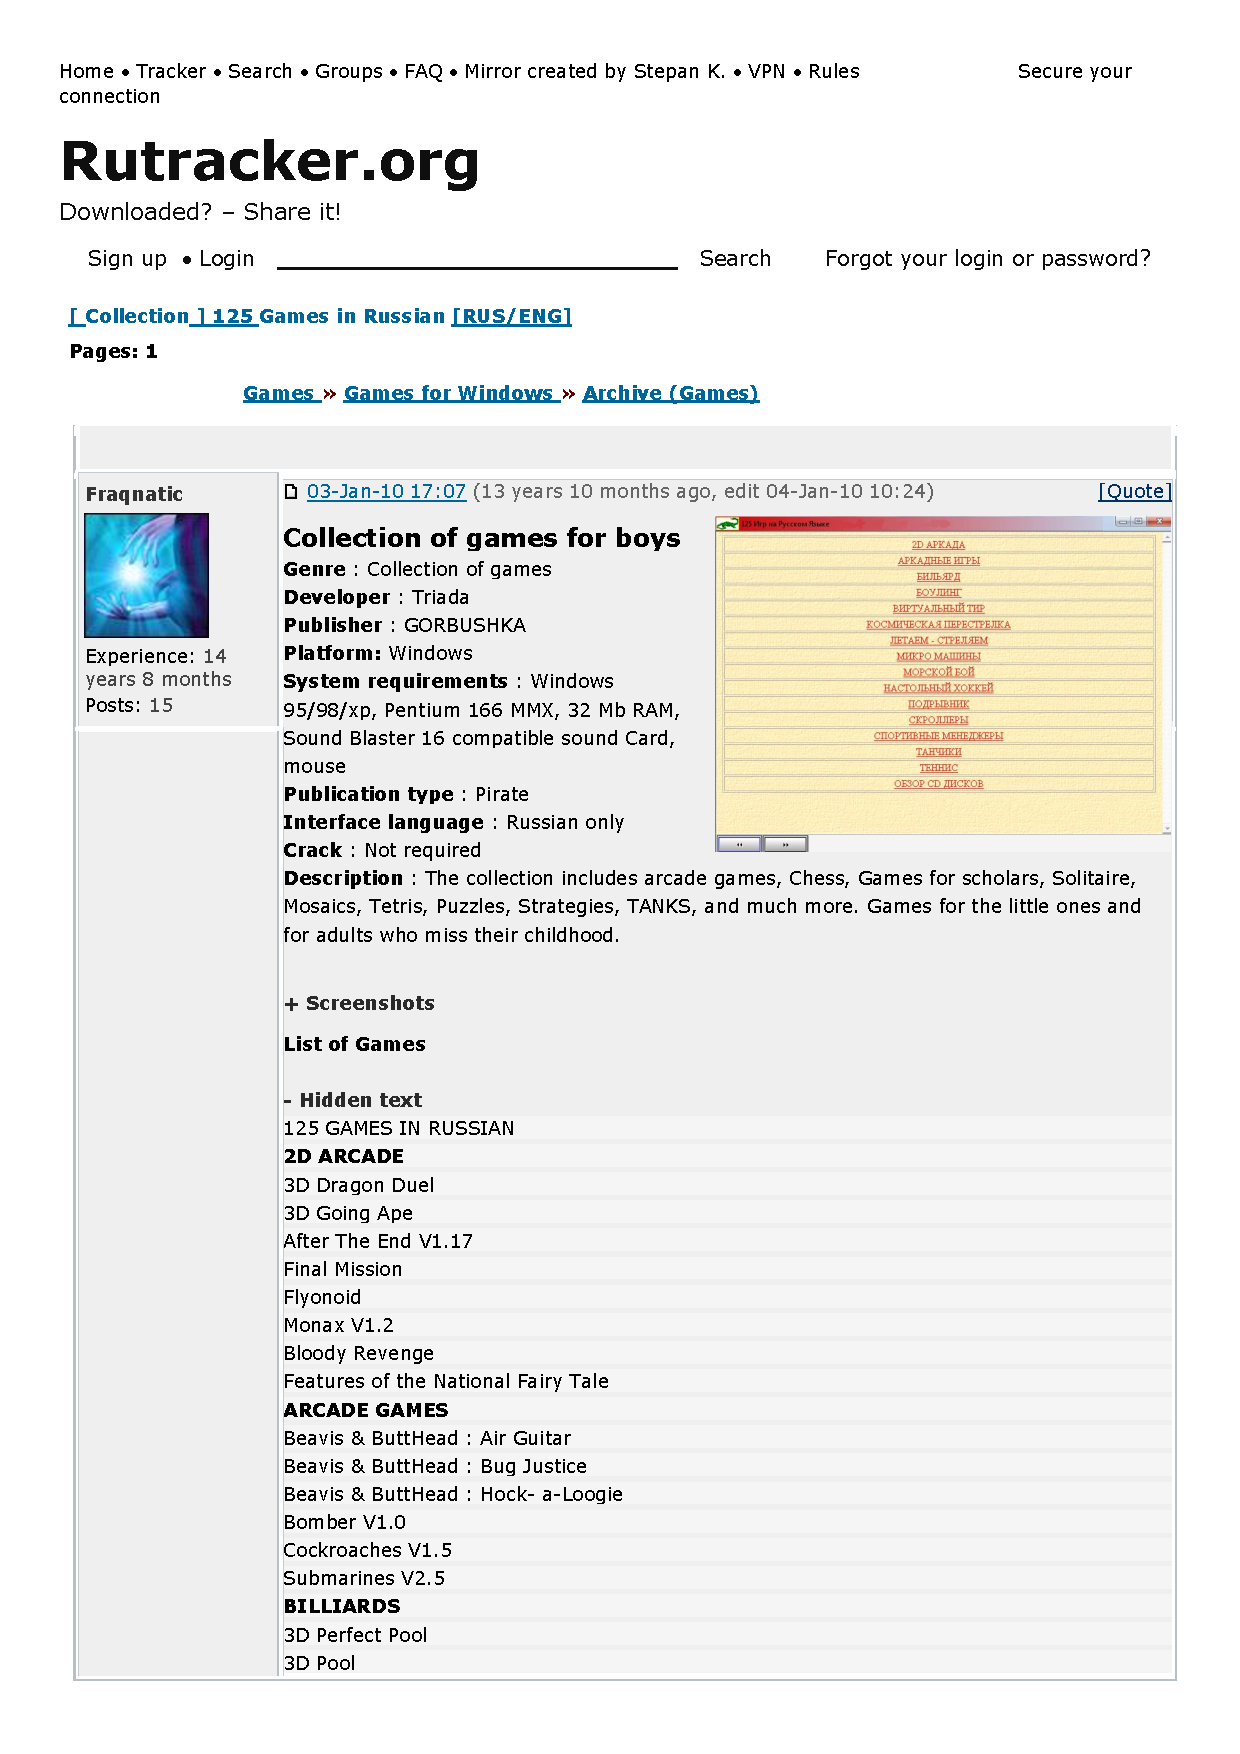
\includepdf[pages=-]{boys_eng_public}

\begin{center}
    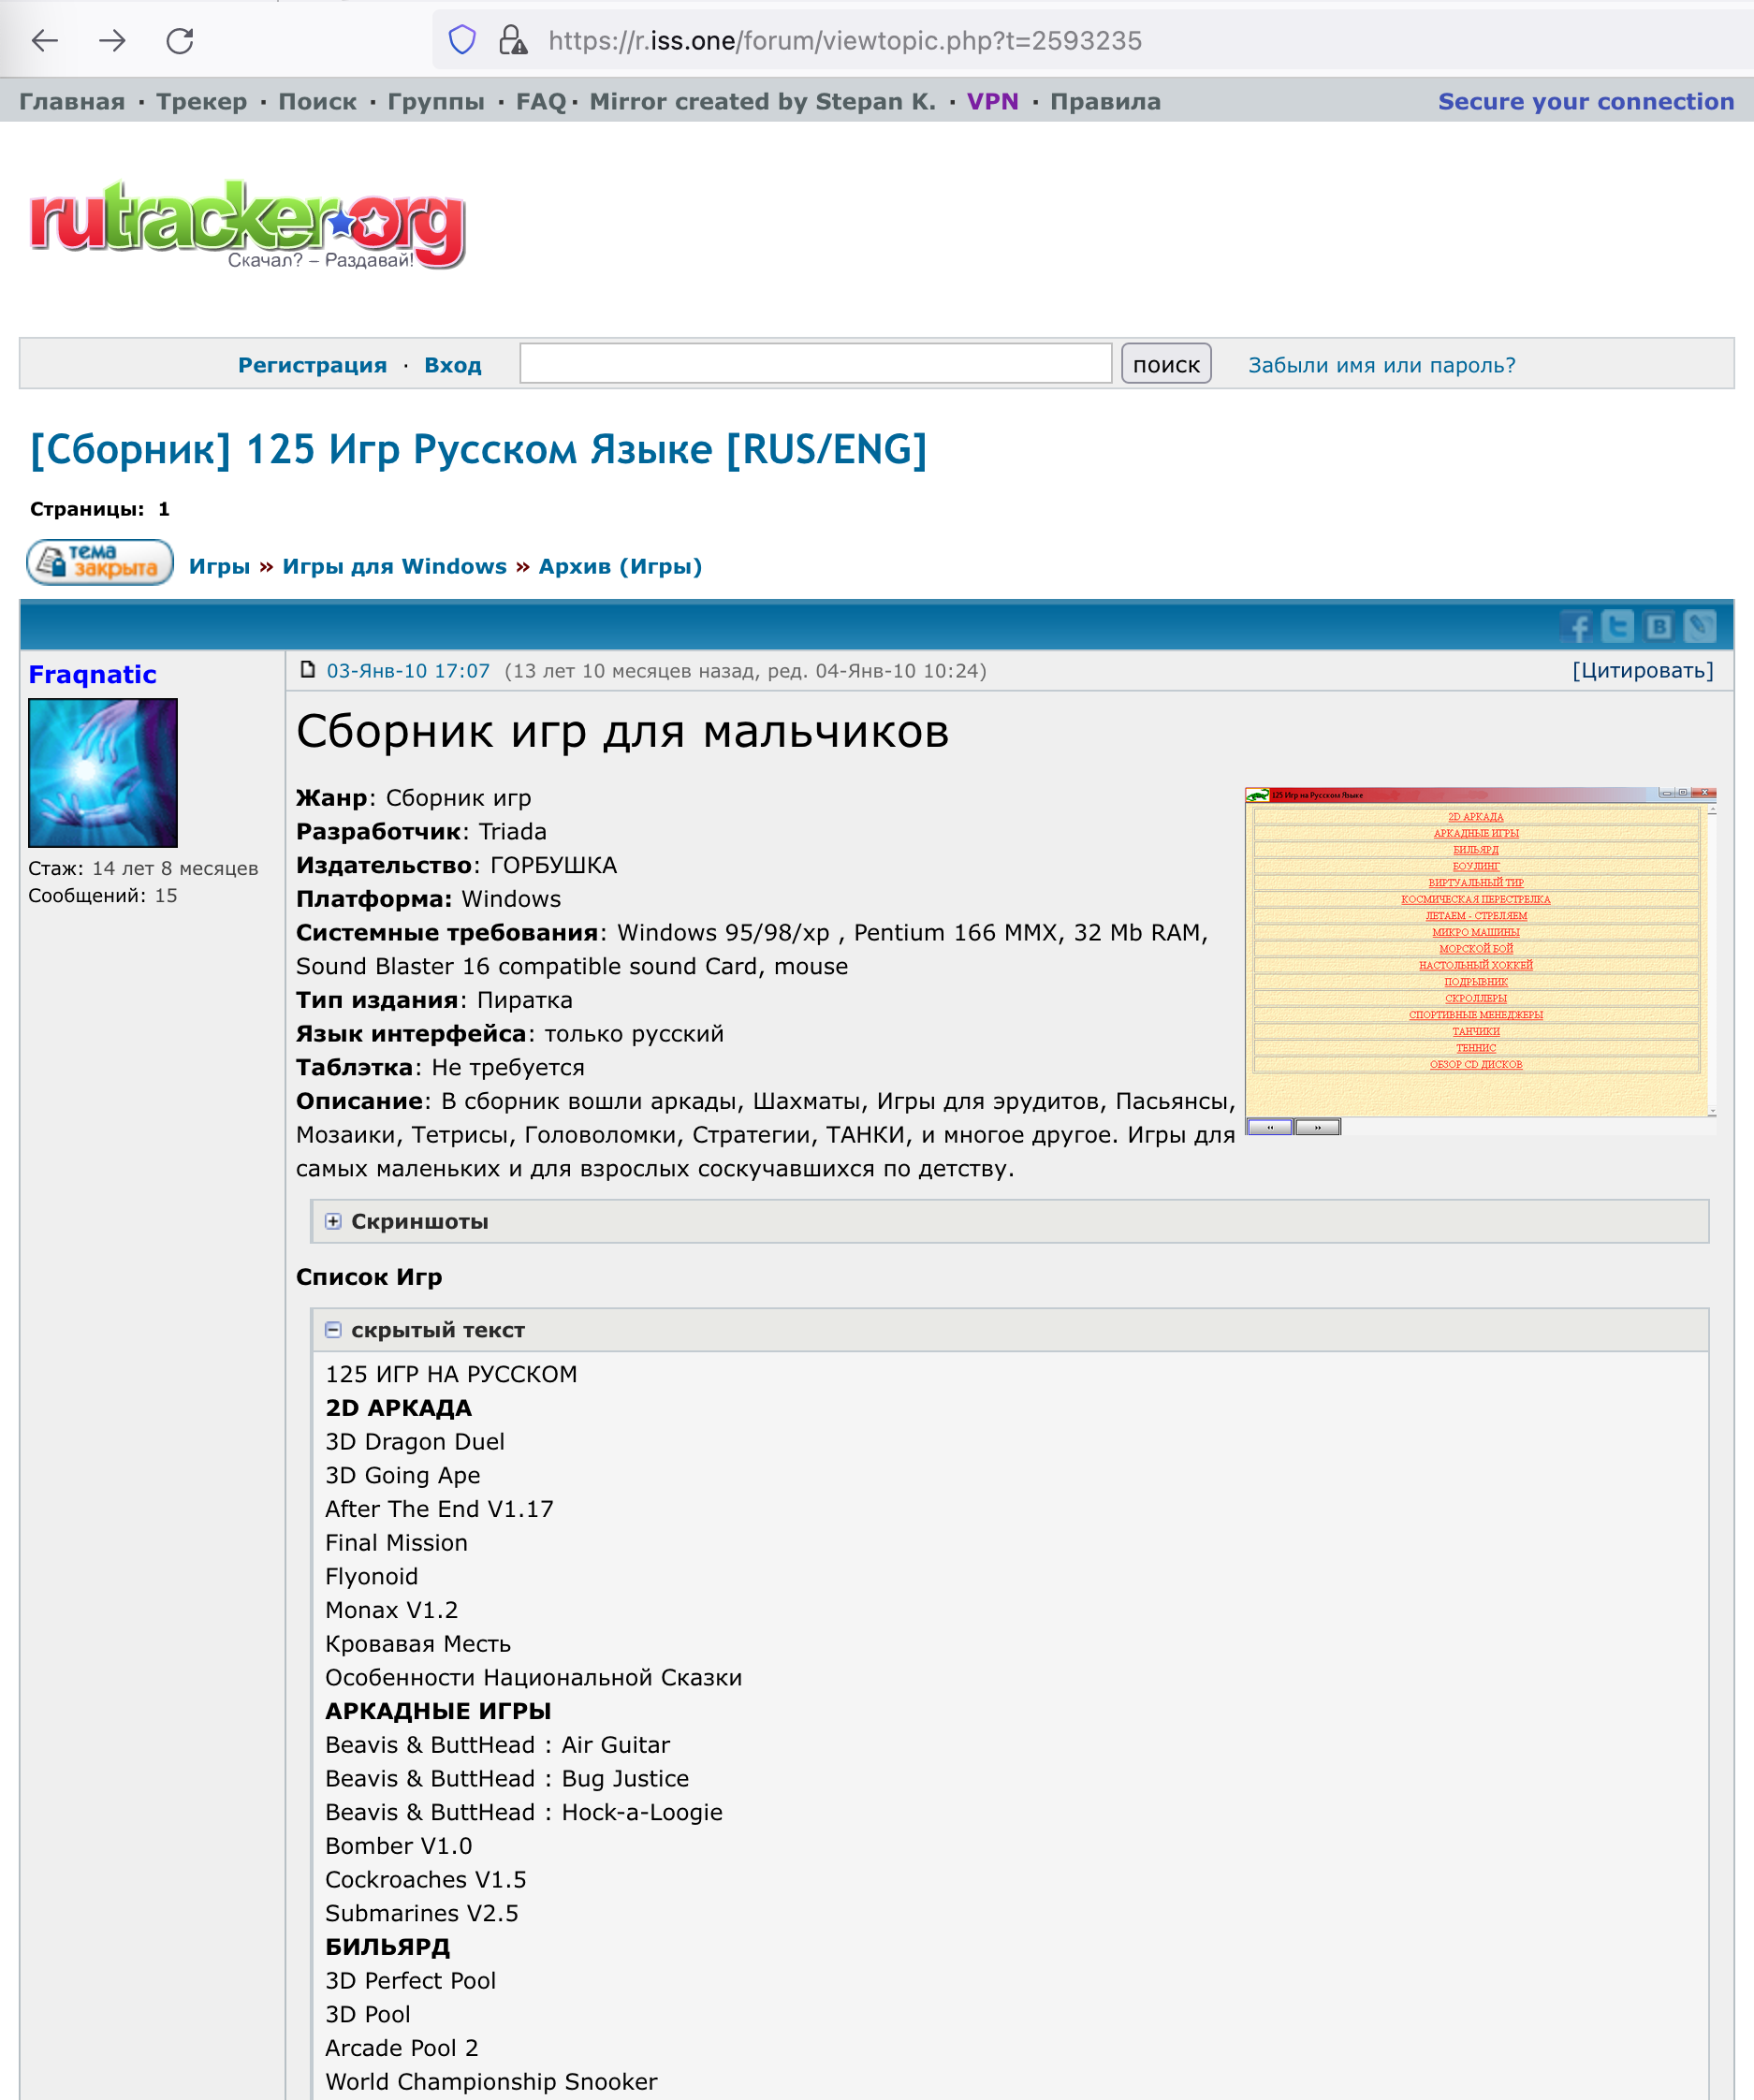
\includegraphics[width=41em]{boys-p1}
\end{center}
\WillContinue
\pagebreak

\Continuing
\begin{center}
    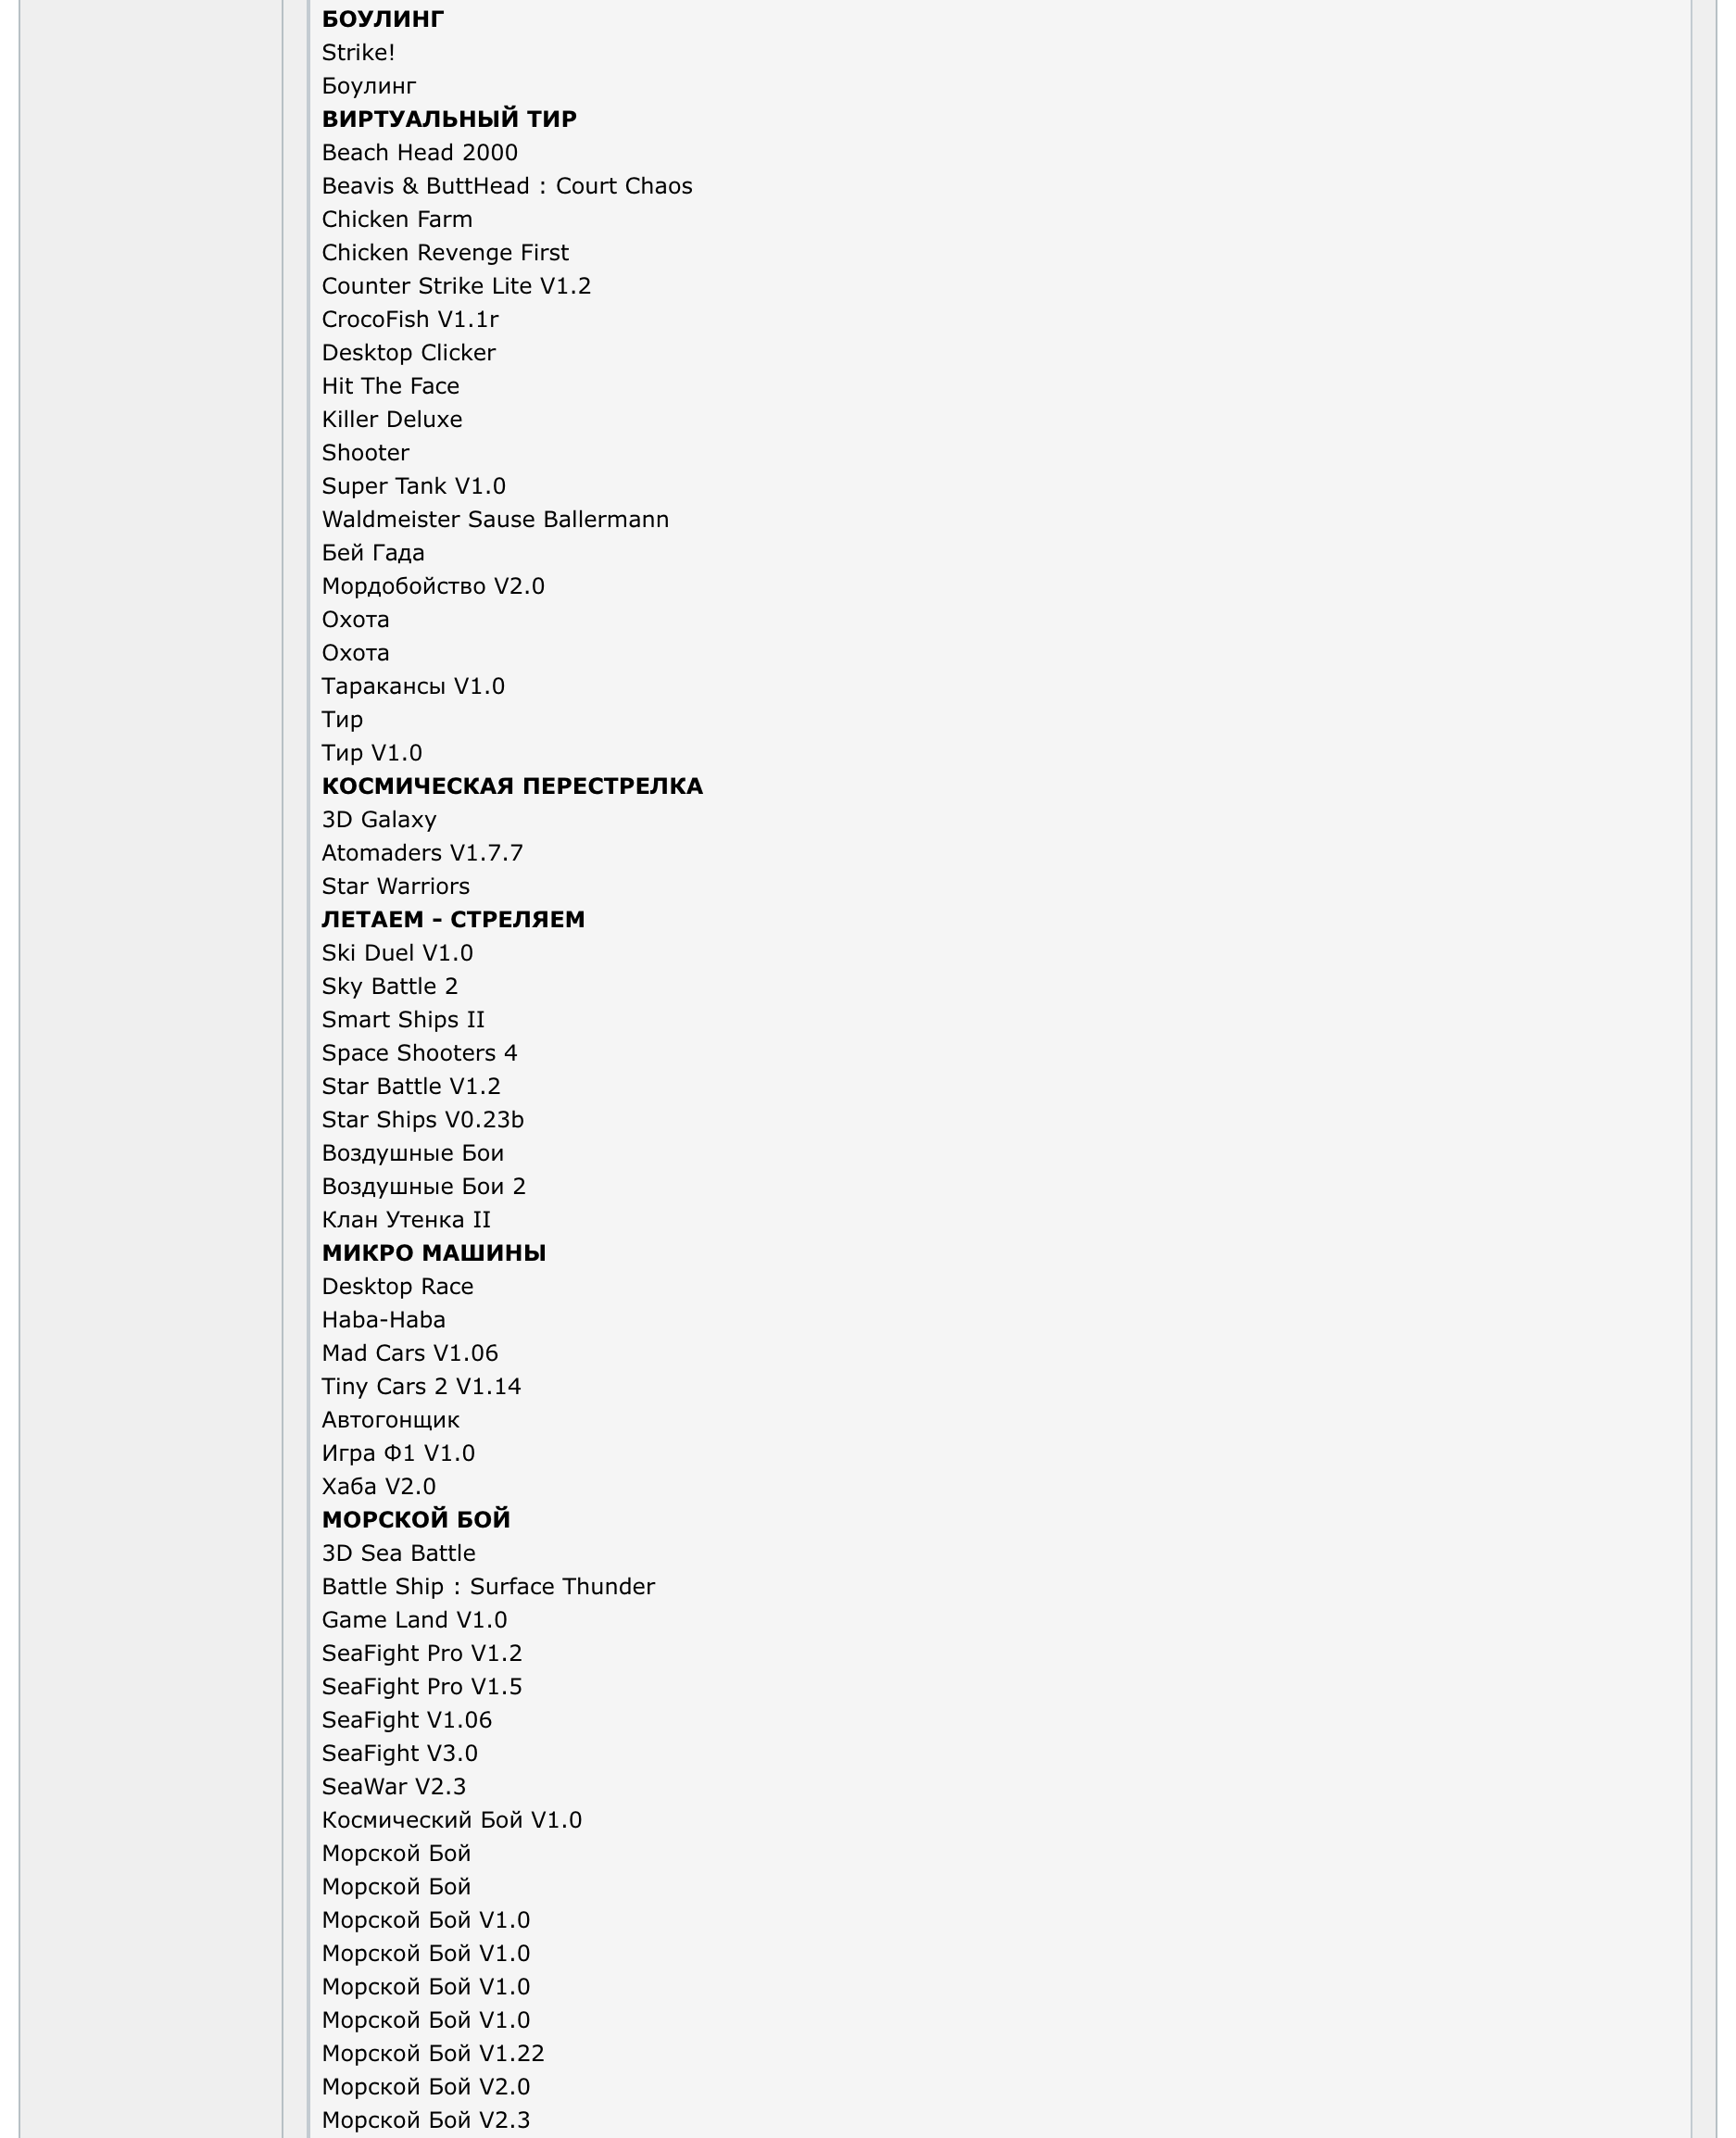
\includegraphics[width=41em]{boys-p2}
\end{center}
\WillContinue
\pagebreak

\Continuing
\begin{center}
    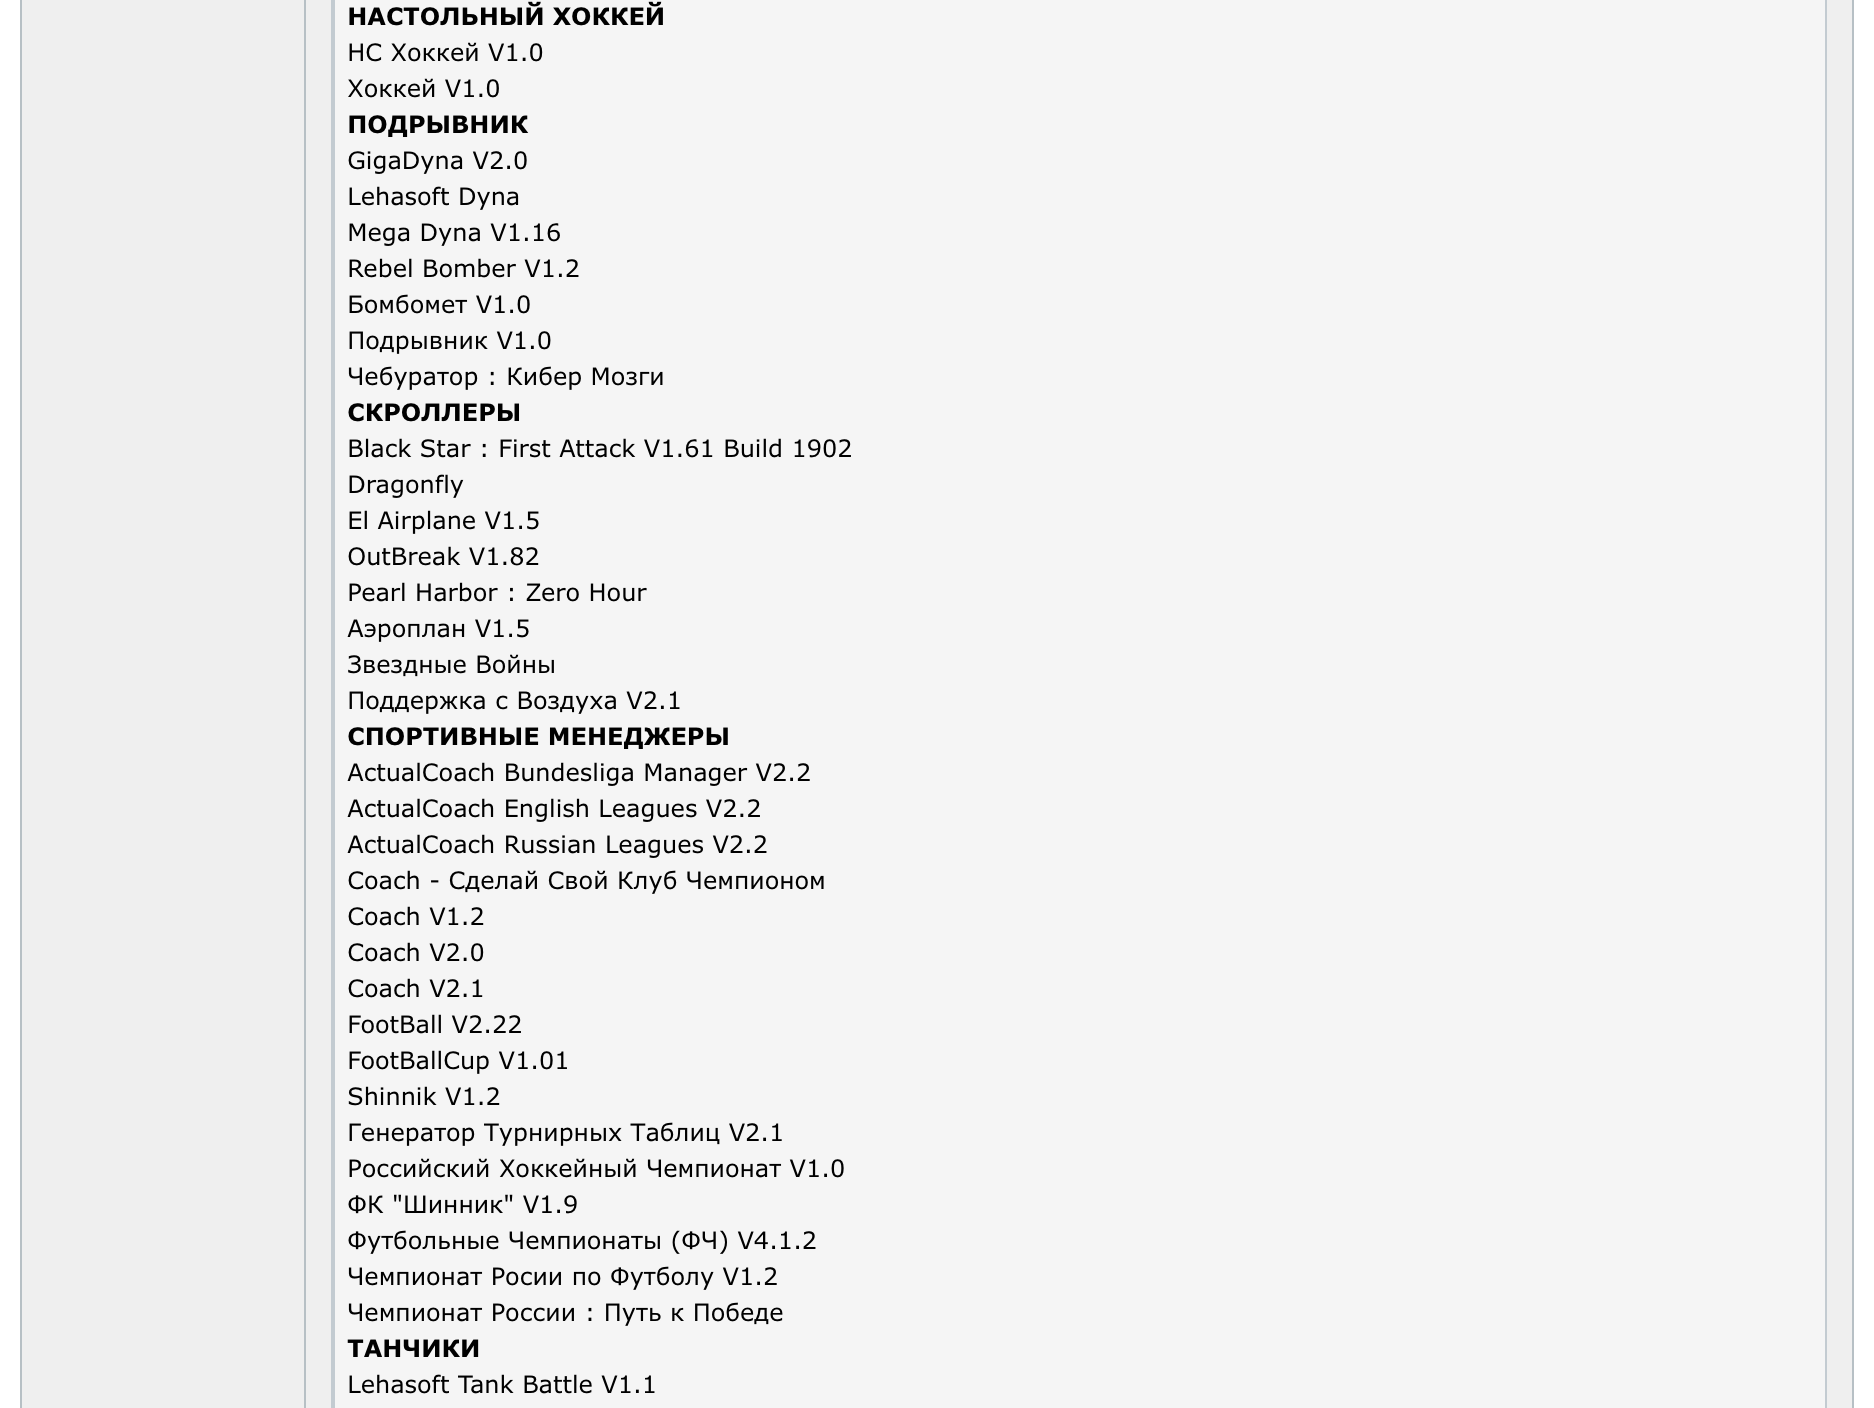
\includegraphics[width=41em]{boys-p3}
\end{center}

\pagebreak
